\documentclass{article}
\usepackage{tikz}
\usepackage{verbatim}
\usetikzlibrary{shapes}
\usetikzlibrary{math}
\usetikzlibrary{decorations.pathreplacing}

\begin{document}
\subsection*{Section of a Normal Column}

\bigskip

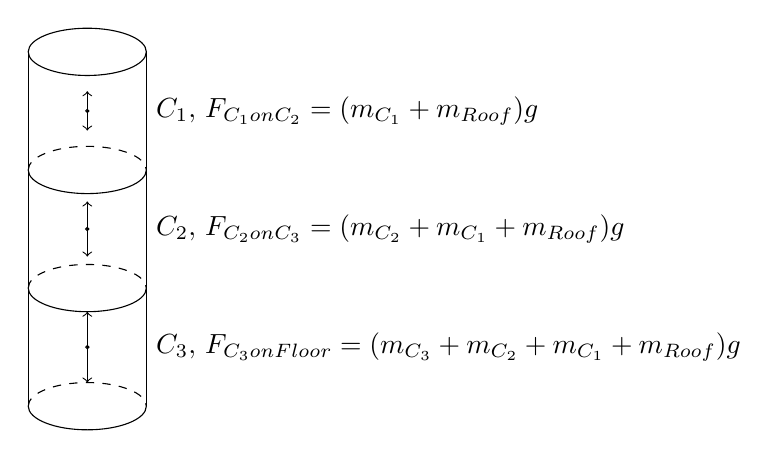
\begin{tikzpicture}[scale = 1]
	    
    \tikzmath{\x1 = -1.5;};
    \tikzmath{\x2 = 0;};
    \tikzmath{\x3 = .25;};
    \draw (.75,\x2) arc (0:360:.75 and 0.3);
	\draw (-.75,\x2) -- (-.75,\x1);
	\draw (-.75,\x1) arc (180:360:.75 and 0.3);
	\draw [dashed] (-.75,\x1) arc (180:360:.75 and -0.3);
	\draw (.75,\x1) -- (.75,\x2);
	  
	\draw [->] (0,\x2 + -.75) -- (0,\x2 + -.75 + \x3);
	\draw (0,\x2 + -.75) circle (.02);
	\node[right] at (.75,\x2 + -.75) {$C_1,$ $F_{C_1 on C_2}=(m_{C_1}+m_{Roof})g$};
	\draw [->] (0,\x2 + -.75) -- (0,\x2 + -.75 - \x3);

	\tikzmath{\x1 = -3;};
    \tikzmath{\x2 = -1.5;};
    \tikzmath{\x3 = .35;};
	\draw (-.75,\x2) -- (-.75,\x1);
	\draw (-.75,\x1) arc (180:360:.75 and 0.3);
	\draw [dashed] (-.75,\x1) arc (180:360:.75 and -0.3);
	\draw (.75,\x1) -- (.75,\x2);
	
	\draw [->] (0,\x2 + -.75) -- (0,\x2 + -.75 + \x3);
	\draw (0,\x2 + -.75) circle (.02);
	\node[right] at (.75,\x2 + -.75) {$C_2,$ $F_{C_2 on C_3}=(m_{C_2}+m_{C_1}+m_{Roof})g$};
	\draw [->] (0,\x2 + -.75) -- (0,\x2 + -.75 - \x3);	
	
	\tikzmath{\x1 = -4.5;};
    \tikzmath{\x2 = -3;};
    \tikzmath{\x3 = .45;};
	\draw (-.75,\x2) -- (-.75,\x1);
	\draw (-.75,\x1) arc (180:360:.75 and 0.3);
	\draw [dashed] (-.75,\x1) arc (180:360:.75 and -0.3);
	\draw (.75,\x1) -- (.75,\x2);
	
	\draw [->] (0,\x2 + -.75) -- (0,\x2 + -.75 + \x3);
	\draw (0,\x2 + -.75) circle (.02);
	\node[right] at (.75,\x2 + -.75) {$C_3,$ $F_{C_3 on Floor}=(m_{C_3}+m_{C_2}+m_{C_1}+m_{Roof})g$};
	\draw [->] (0,\x2 + -.75) -- (0,\x2 + -.75 - \x3);  
	

    
\end{tikzpicture}

\subsection*{Section of a Pushed Column (Low Friction)}
$F_g$ is not shown but acts on all 3 columns on top of the forces already depicted.
\bigskip

\noindent
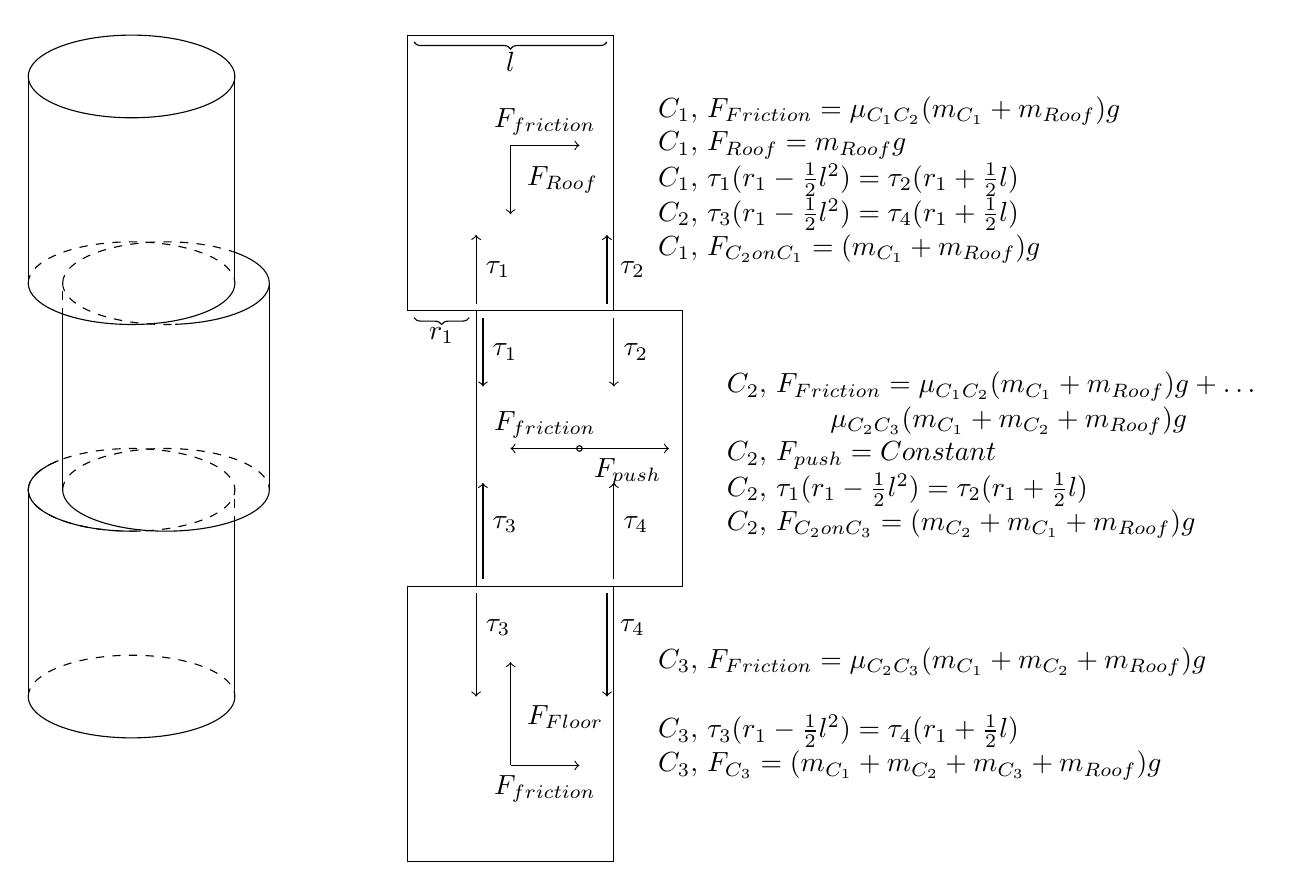
\begin{tikzpicture}[scale = 1.75]
	    
    \tikzmath{\x1 = -1.5;};
    \tikzmath{\x2 = 0;};
    \tikzmath{\x3 = .25;};
    \draw (.75,\x2) arc (0:360:.75 and 0.3);
	\draw (-.75,\x2) -- (-.75,\x1);
	\draw (-.75,\x1) arc (180:360:.75 and 0.3);
	\draw [dashed] (-.75,\x1) arc (180:360:.75 and -0.3);
	\draw (.75,\x1) -- (.75,\x2);
	  
	%\draw [->] (0,\x2 + -.75) -- (0,\x2 + -.75 + \x3);
	%\draw (0,\x2 + -.75) circle (.02);
	% \node [right] at (1,\x2 + -.75) {$C_1,$ $F_{C_1 on C_2}=(m_{C_1}+m_{Roof})g$};
	%\draw [->] (0,\x2 + -.75) -- (0,\x2 + -.75 - \x3);

	\tikzmath{\x1 = -3;};
    \tikzmath{\x2 = -1.5;};
    \tikzmath{\x3 = .35;};
	\draw (-.5,\x2-.24) -- (-.5,\x1);
	\draw [dashed] (-.5,\x2-.24) -- (-.5,\x2);
	\draw (-.5,\x1) arc (180:360:.75 and 0.3);
	\draw [dashed] (-.5,\x1) arc (180:360:.75 and -0.3);
	\draw [dashed] (-.5,\x2) arc (180:275:.75 and 0.3);
	\draw [dashed] (-.5,\x2) arc (180:310:.75 and -0.3);
	\draw (1,\x2) arc (360:310:.75 and -0.3);
	\draw (1,\x2) arc (360:275:.75 and 0.3);
	\draw (1,\x1) -- (1,\x2);
	
	\draw (-.75,\x1) arc (180:275:.75 and 0.3);
	\draw (-.75,\x1) arc (180:225:.75 and -0.3);	
	\draw [dashed] (-.75,\x1) arc (180:360:.75 and 0.3);
	\draw [dashed] (-.75,\x1) arc (180:360:.75 and -0.3);	
	
	%\draw [->] (.25,\x2 + -.75) -- (.5,\x2 + -.75);
	%\draw (.25,\x2 + -.75) circle (.02);
	% \node [right] at (1,\x2 + -.75) {$C_2,$ $F_{C_2 on C_3}=(m_{C_2}+m_{C_1}+m_{Roof})g$};
	%\draw [->] (.25,\x2 + -.75) -- (.25,\x2 + -.75 - \x3);	
	
	\tikzmath{\x1 = -4.5;};
    \tikzmath{\x2 = -3;};
    \tikzmath{\x3 = .45;};
	\draw (-.75,\x2) -- (-.75,\x1);
	\draw (-.75,\x1) arc (180:360:.75 and 0.3);
	\draw [dashed] (-.75,\x1) arc (180:360:.75 and -0.3);
	\draw (.75,\x1) -- (.75,\x2-.25);
	\draw [dashed] (.75,\x2-.25) -- (.75,\x2);
	
	%\draw [->] (0,\x2 + -.75) -- (0,\x2 + -.75 + \x3);
	%\draw (0,\x2 + -.75) circle (.02);
	% \node [right] at (1,\x2 + -.75) {$C_3,$ $F_{C_3 on Floor}=(m_{C_3}+m_{C_2}+m_{C_1}+m_{Roof})g$};
	%\draw [->] (0,\x2 + -.75) -- (0,\x2 + -.75 - \x3);  
	\tikzmath{\x1 = .25;};	
	\draw (2,0.3) rectangle (3.5,-1.7);
	\draw (\x1+2.25,-1.7) rectangle (\x1+3.75,-3.7);
	\draw (2,-3.7) rectangle (3.5,-5.7);
	

	
	\draw [->] (\x1+2.3,-3.65) -- (\x1+2.3,-2.95);
	\draw[decoration={brace,mirror,raise=5pt},decorate] (2.05,-1.65) -- node[below=5pt] {$r_1$} (2.45,-1.65);
	\draw[decoration={brace,mirror,raise=5pt},decorate] (2.05,.35) -- node[below=5pt] {$l$} (3.45,.35);

	\draw [->] (3.5,-3.65) -- (3.5,-2.95);
	\draw [->] (\x1+2.3,-1.75) -- (\x1+2.3,-2.25);
	\node [right] at (\x1+2.3,-2){$\tau_{1}$};
	\node [right] at (\x1+3.25,-2){$\tau_{2}$};
	\node [right] at (\x1+2.3,-3.25){$\tau_{3}$};
	\node [right] at (\x1+3.25,-3.25){$\tau_{4}$};
	\draw [->] (3.5,-1.75) -- (3.5,-2.25);
	\draw [->] (\x1+3,-2.7) -- (\x1+2.5,-2.7);
	\node [above] at (\x1+2.75,-2.7){$F_{friction}$};
	\draw [->] (\x1+3,-2.7) -- (\x1+3.65,-2.7);
	\node [below] at (\x1+3.35,-2.7){$F_{push}$};
	\draw (\x1+3,-2.7) circle (0.02);
	
	\node[right] at (4.25,\x2 + 0.75) {$C_2,$ $F_{Friction}=\mu_{C_1C_2}(m_{C_1}+m_{Roof})g+\dots$};
	\node[right] at (5,\x2 + 0.5) {$\mu_{C_2C_3}(m_{C_1}+m_{C_2}+m_{Roof})g$};
	\node[right] at (4.25,\x2 + 0.25) {$C_2,$ $F_{push}=Constant$};
	\node[right] at (4.25,\x2 + 0) {$C_2,$ $\tau_{1}(r_1-\frac{1}{2}l^2)=\tau_2(r_1+\frac{1}{2}l)$};
	\node[right] at (4.25,\x2 + -.25) {$C_2,$ $F_{C_2 on C_3}=(m_{C_2}+m_{C_1}+m_{Roof})g$};	
	
	\draw [->] (\x1+2.25,-1.65) -- (\x1+2.25,-1.15);
	\draw [->] (3.45,-1.65) -- (3.45,-1.15);
	\draw [->] (2.75,-.5) -- (2.75,-1);
	\node [right] at (2.8,-.75){$F_{Roof}$};	
	\node [right] at (\x1+2.25,-1.4){$\tau_{1}$};
	\node [right] at (3.475,-1.4){$\tau_{2}$};
	\draw [->] (2.75,-.5) -- (3.25,-.5);
	\node [above] at (3,-.5){$F_{friction}$};
	
	\node[right] at (3.75,\x2 + 2.75) {$C_1,$ $F_{Friction}=\mu_{C_1C_2}(m_{C_1}+m_{Roof})g$};
	\node[right] at (3.75,\x2 + 2.5) {$C_1,$ $F_{Roof}=m_{Roof}g$};
	\node[right] at (3.75,\x2 + 2.25) {$C_1,$ $\tau_{1}(r_1-\frac{1}{2}l^2)=\tau_2(r_1+\frac{1}{2}l)$};
	\node[right] at (3.75,\x2 + 2) {$C_2,$ $\tau_{3}(r_1-\frac{1}{2}l^2)=\tau_4(r_1+\frac{1}{2}l)$};
	\node[right] at (3.75,\x2 + 1.75) {$C_1,$ $F_{C_2onC_1}=(m_{C_1}+m_{Roof})g$};
	
	\draw [->] (\x1+2.25,-3.75) -- (\x1+2.25,-4.5);
	\draw [->] (3.45,-3.75) -- (3.45,-4.5);
	\node [right] at (\x1+2.25,-4){$\tau_{3}$};
	\node [right] at (3.475,-4){$\tau_{4}$};
	\draw [->] (2.75,-5) -- (2.75,-4.25);
	\node [right] at (2.8,-4.65){$F_{Floor}$};
	\draw [->] (2.75,-5) -- (3.25,-5);
	\node [below] at (3,-5){$F_{friction}$};
	
	\node[right] at (3.75,\x2 + -1.25) {$C_3,$ $F_{Friction}=\mu_{C_2C_3}(m_{C_1}+m_{C_2}+m_{Roof})g$};
	\node[right] at (3.75,\x2 + -1.75) {$C_3,$ $\tau_{3}(r_1-\frac{1}{2}l^2)=\tau_4(r_1+\frac{1}{2}l)$};
	\node[right] at (3.75,\x2 + -2) {$C_3,$ $F_{C_3}=(m_{C_1}+m_{C_2}+m_{C_3}+m_{Roof})g$};
	
\end{tikzpicture}

\subsection*{Section of a Pushed Column (High Friction) }
$F_g$ is not shown but acts on all 3 columns on top of the forces already depicted. Equations not listed are the same as the low friction model.(4,-2.5)
\bigskip

\noindent
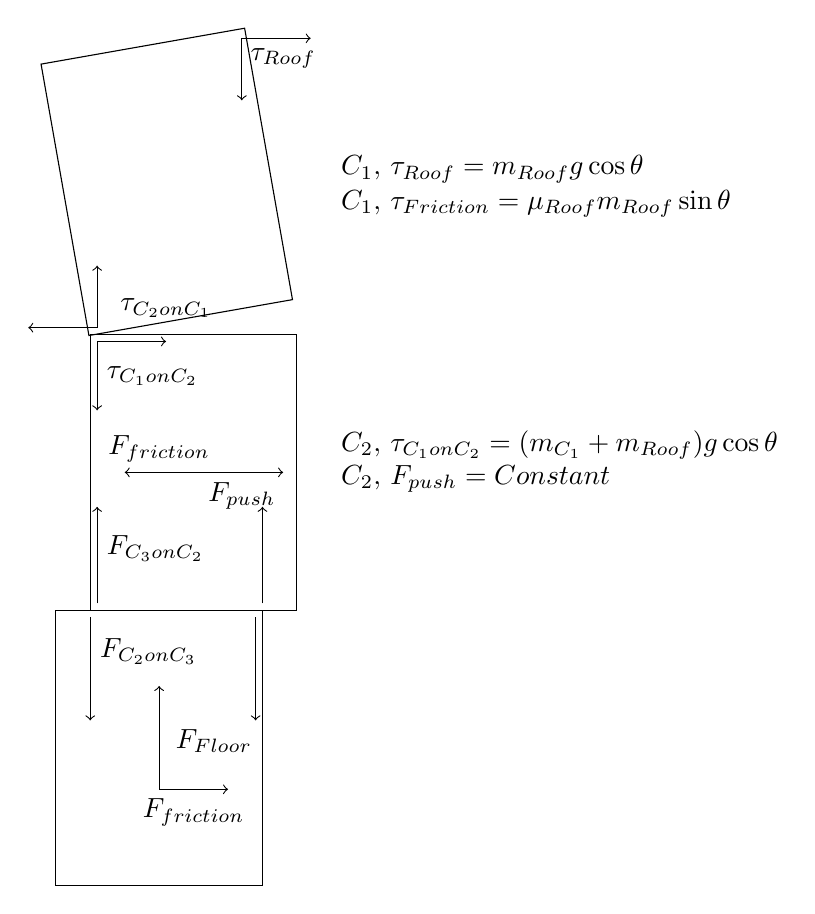
\begin{tikzpicture}[scale = 1.75] 
	
	\draw [rotate=10] (1.91,-0.07) rectangle (3.41,-2.07);
	\draw (2.25,-1.7) rectangle (3.75,-3.7);
	\draw (2,-3.7) rectangle (3.5,-5.7);
	
	\node[right] at (4,-.5) {$C_1,$ $\tau_{Roof}=m_{Roof}g\cos\theta$};
	\node[right] at (4,-.75) {$C_1,$ $\tau_{Friction}=\mu_{Roof}m_{Roof}\sin\theta$};
	
	\node[right] at (4,-2.5) {$C_2,$ $\tau_{C_1onC_2}=(m_{C_1}+m_{Roof})g\cos\theta$};
	\node[right] at (4,-2.75) {$C_2,$ $F_{push}=Constant$};
	
	\draw [->] (2.3,-3.65) -- (2.3,-2.95);
	\node [right] at (2.3,-3.25){$F_{C_3 on C_2}$};
	\draw [->] (3.5,-3.65) -- (3.5,-2.95);
	\draw [->] (2.3,-1.75) -- (2.3,-2.25);
	\draw [->] (2.3,-1.75) -- (2.8,-1.75);
	\node [right] at (2.3,-2){$\tau_{C_1 on C_2}$};
	%\draw [->] (3.5,-1.75) -- (3.5,-2.25);
	\draw [->] (3,-2.7) -- (2.5,-2.7);
	\node [above] at (2.75,-2.7){$F_{friction}$};
	\draw [->] (3,-2.7) -- (3.65,-2.7);
	\node [below] at (3.35,-2.7){$F_{push}$};

	\draw [->] (2.3,-1.65) -- (2.3,-1.2);
	\draw [->] (2.3,-1.65) -- (1.8,-1.65);
	\node [above] at (2.8,-1.65){$\tau_{C_2 on C_1}$};
	\draw [->] (3.35,.45) -- (3.35,0);
	\draw [->] (3.35,.45) -- (3.85,.45);
	\node [below] at (3.65,.45){$\tau_{Roof}$};
	
\begin{comment}
	\draw (3,-2.7) circle (0.02);
	\draw [->] (2.25,-1.65) -- (2.25,-1.15);
	\draw [->] (3.45,-1.65) -- (3.45,-1.15);
	\draw [->] (2.75,-.5) -- (2.75,-1);
	\node [right] at (2.8,-.75){$F_{Roof}$};	
	\node [right] at (2.25,-1.4){$F_{C_2 on C_1}$};
	\draw [->] (2.75,-.5) -- (3.25,-.5);
	\node [above] at (3,-.5){$F_{friction}$};
\end{comment}

	\draw [->] (2.25,-3.75) -- (2.25,-4.5);
	\draw [->] (3.45,-3.75) -- (3.45,-4.5);
	\node [right] at (2.25,-4){$F_{C_2 on C_3}$};
	\draw [->] (2.75,-5) -- (2.75,-4.25);
	\node [right] at (2.8,-4.65){$F_{Floor}$};
	\draw [->] (2.75,-5) -- (3.25,-5);
	\node [below] at (3,-5){$F_{friction}$};

\end{tikzpicture}

\end{document}